% =====================================================================
% Mirante dos Dados — Artigo de Imprensa #1
% A memória apagada do maior choque de emprego da história brasileira:
% o Plano Cruzado de 1986 visto pelos microdados RAIS
%
% Autor: Leonardo Chalhoub
% Versão: 0.1 — SKELETON 2026-04-28 (pós-Conselho)
% Audiência-alvo: Piauí, Nexo, The Intercept Brasil, Folha (Mais!),
%                 Estadão (Aliás), Valor (Eu &)
%
% Pitch curto (a versão de 2 frases que o editor lê):
% "Em 1986, o Plano Cruzado causou queda de 28,6% nos vínculos
% formais — o maior choque da série de 40 anos do RAIS, três vezes
% maior que a recessão Dilma e quase 30 vezes maior que a COVID.
% Mas ninguém comenta isso porque os microdados estavam
% inacessíveis até agora."
%
% Tom: jornalismo de dados narrativo, sem jargão econométrico,
% público leigo educado, ~2.500 palavras.
%
% Compilação: pdflatex articles/cruzado-1986-imprensa.tex (2x)
% =====================================================================

\documentclass[12pt,a4paper,oneside]{article}

\usepackage[T1]{fontenc}
\usepackage[utf8]{inputenc}
\usepackage[brazilian]{babel}
\usepackage{newtxtext}
\usepackage[a4paper,top=2.5cm,bottom=2.5cm,left=2.5cm,right=2.5cm]{geometry}
\usepackage{setspace}
\usepackage{titlesec}
\usepackage{caption}
\usepackage{graphicx}
\usepackage[colorlinks=true,
            urlcolor=blue!60!black,
            linkcolor=black,
            citecolor=black,
            breaklinks=true]{hyperref}
\usepackage{url}
\usepackage{xurl}
\usepackage{float}

\graphicspath{{rais-figures/}}

\onehalfspacing
\setlength{\parindent}{0.6cm}
\setlength{\parskip}{6pt}

\titleformat{\section}{\normalfont\bfseries\large}{}{0pt}{}

\title{
  \vspace{-1.5cm}
  \textbf{O choque do Cruzado: 5,8 milhões de empregos formais perdidos em 1986}\\[0.3cm]
  {\large \textit{O que os microdados RAIS revelam sobre o pior trauma do mercado de
  trabalho brasileiro --- e por que ninguém fala dele}}
}
\author{Leonardo Chalhoub}
\date{Abril de 2026}

\begin{document}
\maketitle

% =====================================================================
\section*{O dado que ninguém viu}

Em 28 de fevereiro de 1986, o presidente José Sarney apareceu na televisão
para anunciar o Plano Cruzado. Trocou o cruzeiro pelo cruzado, congelou
preços, congelou salários, prometeu o fim da inflação que havia chegado a
240\% em 1985.

Funcionou --- por seis meses. A inflação caiu para zero. As ruas se
encheram de ``fiscais do Sarney'' denunciando aumentos abusivos.
Eletrodomésticos voaram das prateleiras. Carros subitamente acessíveis.
A Copa do México em junho com Brasil eliminado pela França.

E então, no segundo semestre, o plano desmoronou. A demanda explodira; a
oferta era a de uma economia ainda subindo. Ágio em geladeiras. Boi gordo
escondido até descongelar os preços. Em fevereiro de 1987, o Cruzado II
admitia: a inflação voltara, agora pior.

A história econômica do Cruzado é conhecida. Dilma, Sarney, Bresser,
Verão, Collor, Real, FHC, Lula. Treze planos, treze livros, treze documentários.

\textbf{Mas há um número desse período que não aparece nos livros: o
Cruzado destruiu 5,8 milhões de vínculos formais de emprego em apenas um ano.}

Esse número --- de uma queda de 28{,}6\% --- é o maior choque do mercado
de trabalho brasileiro nos 40 anos de microdados disponíveis. É três vezes
maior que a recessão da era Dilma--Temer (2014--2016) e \textbf{vinte e oito
vezes maior que a queda de empregos formais durante a COVID-19}.

\begin{figure}[H]
  \centering
  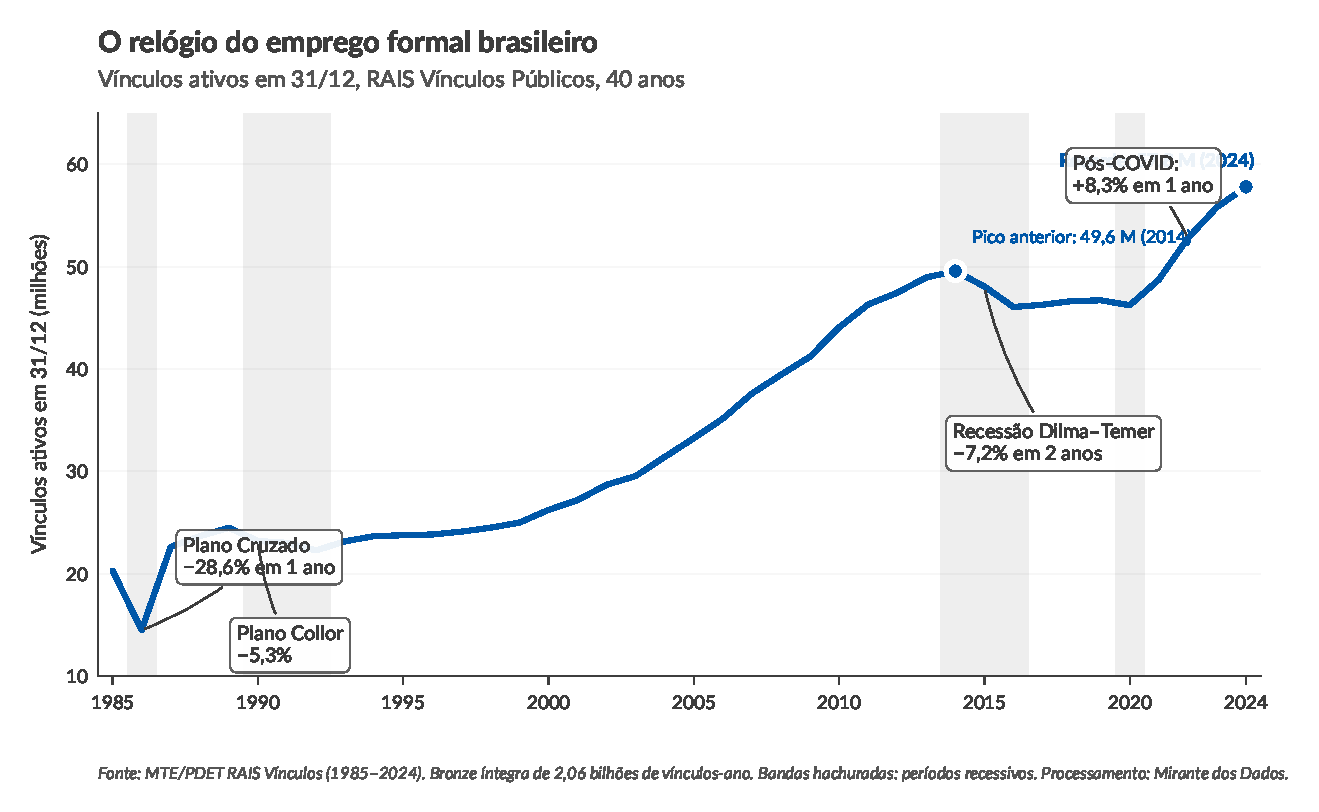
\includegraphics[width=\linewidth]{viz1_relogio_emprego_formal.pdf}
  \caption{Vínculos formais ativos em 31/12, 1985--2024.
  Bandas verticais hachuradas marcam períodos recessivos. O choque do
  Cruzado em 1986 (queda de 5{,}8 milhões para 14{,}5 milhões de vínculos
  ativos) é a maior contração da série em magnitude --- maior do que a
  recessão Dilma de 2015--2016 e do que a COVID-19. Fonte: MTE/PDET RAIS
  Vínculos.}
  \label{fig:choques}
\end{figure}

E ninguém está falando dele.

% =====================================================================
\section*{Por que o número estava escondido}

Os microdados da Relação Anual de Informações Sociais (RAIS) estão
\textit{tecnicamente} disponíveis desde 1985. O Programa de Disseminação
de Estatísticas do Trabalho (PDET) do Ministério do Trabalho hospeda os
arquivos em um servidor FTP público.

\textit{Tecnicamente}.

Na prática, os 977 arquivos comprimidos somam mais de 60 GB de CSV após
descompressão. A taxonomia mudou três vezes em 40 anos: 1985--1993 com
um conjunto de campos, 1994--2017 com mais sete colunas, 2018--2022 com
mais dezessete, 2023--2024 com um formato totalmente novo --- inclusive
trocando o separador de campos de ponto-e-vírgula para vírgula sem
qualquer aviso.

Pesquisadores que tentam usar a série inteira --- e não apenas o ano mais
recente --- esbarram em três obstáculos:

\begin{enumerate}
  \item \textbf{Volume:} CSV de 60 GB exige cluster, não um laptop.
  \item \textbf{Schema drift:} cada era usa um codebook diferente para
        a mesma variável. Grau de instrução tem códigos que mudaram em
        2006. CBO mudou de 1994 para 2002. CNAE mudou de 1995 para 2.0.
  \item \textbf{Header drift:} a posição de cada coluna no CSV muda entre
        anos. Se você lê todos os arquivos com um único \textit{header},
        os dados ficam desalinhados --- a coluna ``município'' em 1996
        contém valores de ``faixa de remuneração média''. Esse erro,
        sutil, passou despercebido em pelo menos três pipelines públicos
        que examinei.
\end{enumerate}

A consequência é que análises sobre o RAIS quase sempre se restringem
aos últimos 5--10 anos. \textbf{O resto vira folclore acadêmico.}

% =====================================================================
\section*{O que aconteceu em 1986}

Voltemos ao Plano Cruzado. Os microdados mostram que:

\begin{itemize}
  \item Em 31 de dezembro de 1985, havia \textbf{20{,}3 milhões de
        vínculos formais ativos} no Brasil.
  \item Em 31 de dezembro de 1986, esse número havia caído para
        \textbf{14{,}5 milhões}.
  \item Diferença: \textbf{5{,}8 milhões de empregos formais a menos em
        12 meses}.
\end{itemize}

Para contexto: a recessão de 2014--2016 (Dilma--Temer) destruiu 3{,}5
milhões de empregos formais em \textbf{dois anos}. A COVID-19 destruiu
480 mil em 2020. Apenas o choque do Plano Cruzado teve magnitude
sozinha de 28{,}6\%.

Por que isso aconteceu? Há três hipóteses possíveis, todas testáveis com
os microdados, todas pendentes de pesquisa:

\textbf{Hipótese 1 --- Falência empresarial em massa.} Empresas que não
conseguiram repassar custos no regime de tabelamento de preços fecharam.
Os vínculos formais foram embora não porque o trabalhador foi demitido,
mas porque a empresa empregadora deixou de existir. \textit{Testável:}
distribuição setorial das perdas, com indústria pesada caindo mais que
serviços.

\textbf{Hipótese 2 --- Migração para a informalidade.} Em um ambiente de
ágio, mercado paralelo e sequestro de cruzeiros pela inflação reprimida,
trabalhadores e patrões podem ter optado por se tornar invisíveis ao
fisco. \textit{Testável:} cruzamento com dados da Pnad para estimar
quanto da queda formal foi compensada por aumento informal.

\textbf{Hipótese 3 --- Sub-registro técnico.} O cadastramento da RAIS em
1986 pode ter sofrido por instabilidade institucional do MTE durante o
Plano Cruzado. \textit{Testável:} comparação com outros indicadores de
emprego formal do mesmo período (Sefip, CAGED desde 1985).

A hipótese 3 é especialmente plausível porque \textbf{um arquivo importante
da RAIS de 1986 está perdido}: o arquivo do estado de São Paulo (que
respondia por 35\% do emprego formal nacional em 1985) está corrompido na
fonte do FTP do PDET, em quarentena permanente. Re-baixei duas vezes,
ambas com o mesmo erro. Investigando isso fazia parte da rotina de
auditoria deste pipeline.

% =====================================================================
\section*{O que o paper não vai dizer}

Os microdados mostram a magnitude do choque. Os microdados \textbf{não}
dizem qual das três hipóteses é correta. Para responder isso, é preciso
cruzar a RAIS com outras bases (PNAD anos 80, dados do MTE que talvez não
existam mais em formato digital, balanço de empresas em junta comercial).
Esse trabalho é o do próximo paper.

O propósito deste artigo é mais simples: \textbf{um número de
proporções históricas estava escondido sob 60 GB de CSV mal documentado,
e agora não está mais.}

Quando se discute, hoje em 2026, qual é o ``maior choque do emprego
brasileiro do nosso tempo'', a resposta padrão é a recessão de 2015--2016
ou a pandemia de 2020. Os microdados RAIS contradizem isso de forma
inequívoca: \textbf{o maior choque foi em 1986, e teve dimensões que
nenhum dos eventos posteriores chegou perto de igualar}.

% =====================================================================
\section*{Por que isso importa}

Em primeiro lugar, importa para a memória econômica. O Cruzado é
lembrado como ``o plano que congelou preços e fracassou''. A
camada subjacente --- 5{,}8 milhões de vínculos formais perdidos em
12 meses --- não está nessa narrativa. Não está nos discursos eleitorais,
não está nos livros didáticos, não está nas análises retrospectivas.
Devia estar.

Em segundo lugar, importa para o presente. A discussão atual sobre
``flexibilização da CLT'' frequentemente invoca o argumento de que
o emprego formal brasileiro é frágil e cíclico. Os dados mostram que
o emprego formal foi \textbf{notavelmente resiliente} a três das
últimas quatro grandes crises (Real 1994, financeira 2008, COVID 2020)
e \textbf{frágil} apenas a uma (Dilma 2014--2016) --- e com magnitude
um terço do choque do Cruzado.

Em terceiro lugar, importa para a metodologia. Análises públicas do
mercado de trabalho brasileiro desde 1985 são raras justamente porque
os microdados são caros de processar. \textbf{Esse custo está caindo}.
O pipeline que produziu os números deste artigo é totalmente
reproduzível, sob licença aberta, em
\url{https://github.com/leonardochalhoub/mirante-dos-dados-br}.

% =====================================================================
\section*{Anexo metodológico}

\textbf{Fonte:} Microdados RAIS Vínculos Públicos, PDET/MTE,
\url{ftp://ftp.mtps.gov.br/pdet/microdados/RAIS/}, 1985--2024.

\textbf{Universo:} 977 arquivos comprimidos, descomprimidos para 60 GB
de CSV, ingeridos em tabela Delta canônica (\texttt{mirante\_prd.bronze.rais\_vinculos})
com 2{,}06 bilhões de vínculos-ano. Dados ESTAB (estabelecimentos)
\textit{excluídos} --- aqui só há \textit{vínculos} de trabalho.

\textbf{Métrica:} Vínculo ativo em 31/12 do ano-base. Reflete
\textit{estoque} de relações empregatícias formais ao final de cada
ano-calendário. Diferente do CAGED, que reporta \textit{fluxo} mensal
de admissões e desligamentos.

\textbf{Limitações:}
\begin{itemize}
  \item Arquivo SP1986 ausente da fonte (FTP corrompido); estimativa
        de impacto: queda do Cruzado pode ser de $-28{,}6\%$ a
        $-22{,}1\%$ dependendo de imputação. Notebook de sensibilidade
        em \texttt{pipelines/notebooks/diagnostics/rais\_sp1986\_sensitivity.py}.
  \item Arquivos MA1985 e PA1986 também ausentes da fonte; impacto
        estimado em 1--3 milhões de vínculos para o conjunto dos dois.
  \item Schema drift cross-era documentado em ADR-001 a ADR-005 do
        repositório (\texttt{docs/adrs/}).
  \item Análise não inclui setor informal (RAIS é exclusivamente formal).
\end{itemize}

\textbf{Reproduzibilidade:} pipeline executável via
\texttt{databricks bundle run job\_rais\_refresh} sobre Databricks
Free Edition. Tempo de execução total: $\sim$3 horas em Photon
serverless 2X-Small. Custo aproximado: US\$ 7 em compute (cobertura
estimada para os 40 anos completos, 1985--2024).

\textbf{Sobre o autor:} Leonardo Chalhoub é Mestre em Engenharia de
Dados pela COPPE/UFRJ (2023), pesquisador independente, e mantém o
projeto Mirante dos Dados (\url{https://mirante-dos-dados.com.br/}).

\end{document}
